\hypertarget{fence-automated-testing-environment}{%
\section{Fate e desenvolvimento de testes ponta a ponta}\label{fence-automated-testing-environment}}

O \emph{Fence Automated Testing Environment}, ou apenas \emph{Fate}, possui o objetivo de testar as interfaces de um sistema web de acordo com os seus requisitos. Como presente de forma simplificada na figura \ref{fig:fate-esq}, o \emph{Fate} é um \emph{framework} para testes \emph{end-to-end}, ou \emph{e2e}, e utiliza como entrada os requisitos expressos no plano de testes, e com os testes desenvolvidos a partir dele, o relatório de erros é gerado.

\begin{figure}[H]
    \centering
    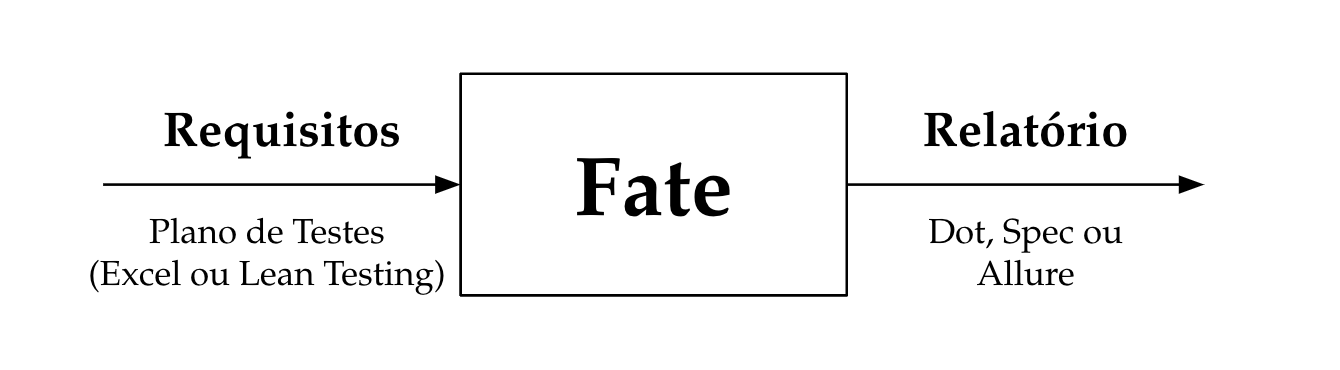
\includegraphics[width=13cm]{source/4-solucao/images/fate-esq.png}
    \caption{Simplificação do \emph{Fate}. A partir de um plano de testes, um relatório final com \emph{test cases} é gerado.}
    \label{fig:fate-esq}
\end{figure}

Esta seção foca desde as experiências realizadas inicialmente com diversas ferramentas \emph{end-to-end} até a escolha final. Após isso é detalhado as características da ferramenta escolhida e o planejamento do \emph{framework} \emph{Fate}, descrevendo as tecnologias utilizadas e casos de uso.

\hypertarget{escolha-de-ferramenta-e2e}{%
\subsubsection{\texorpdfstring{Escolha de ferramenta \emph{end-to-end}}{Escolha de ferramenta e2e}}\label{escolha-de-ferramenta-e2e}}

Diferentemente do \emph{phpunit}, não existe a consolidação na comunidade de uma ferramenta para \emph{end-to-end testing}. Mais de dez diferentes tecnologias foram avaliadas durante a realização deste trabalho.

Inicialmente para o desenvolvimento de um protótipo, foram experimentadas duas ferramentas simultaneamente, \emph{Sikuli} e \emph{Selenium IDE}, com exemplos de código na figura \ref{fig:e2e-ferramenta}. \emph{Sikuli}, atualmente chamado de \emph{SikuliX}, se trata de um \emph{framework} no qual é possível utilizar capturas de tela, ou \emph{screenshots}, de elementos da página juntamente com sua lógica, em uma abordagem diferente das outras ferramentas. Já o \emph{Selenium IDE}, que faz parte da coleção \emph{Selenium} de ferramentas de automação de navegadores, se baseia no conceito de \emph{capture and replay}, no qual o testador realiza os comandos no navegador e o \emph{Selenium IDE} captura estas iterações, gerando o código referente aos eventos e aos elementos da página web. Na imagem \ref{fig:e2e-ferramenta} é possível ver exemplo destas ferramentas.

\begin{figure}[H]
    \centering
    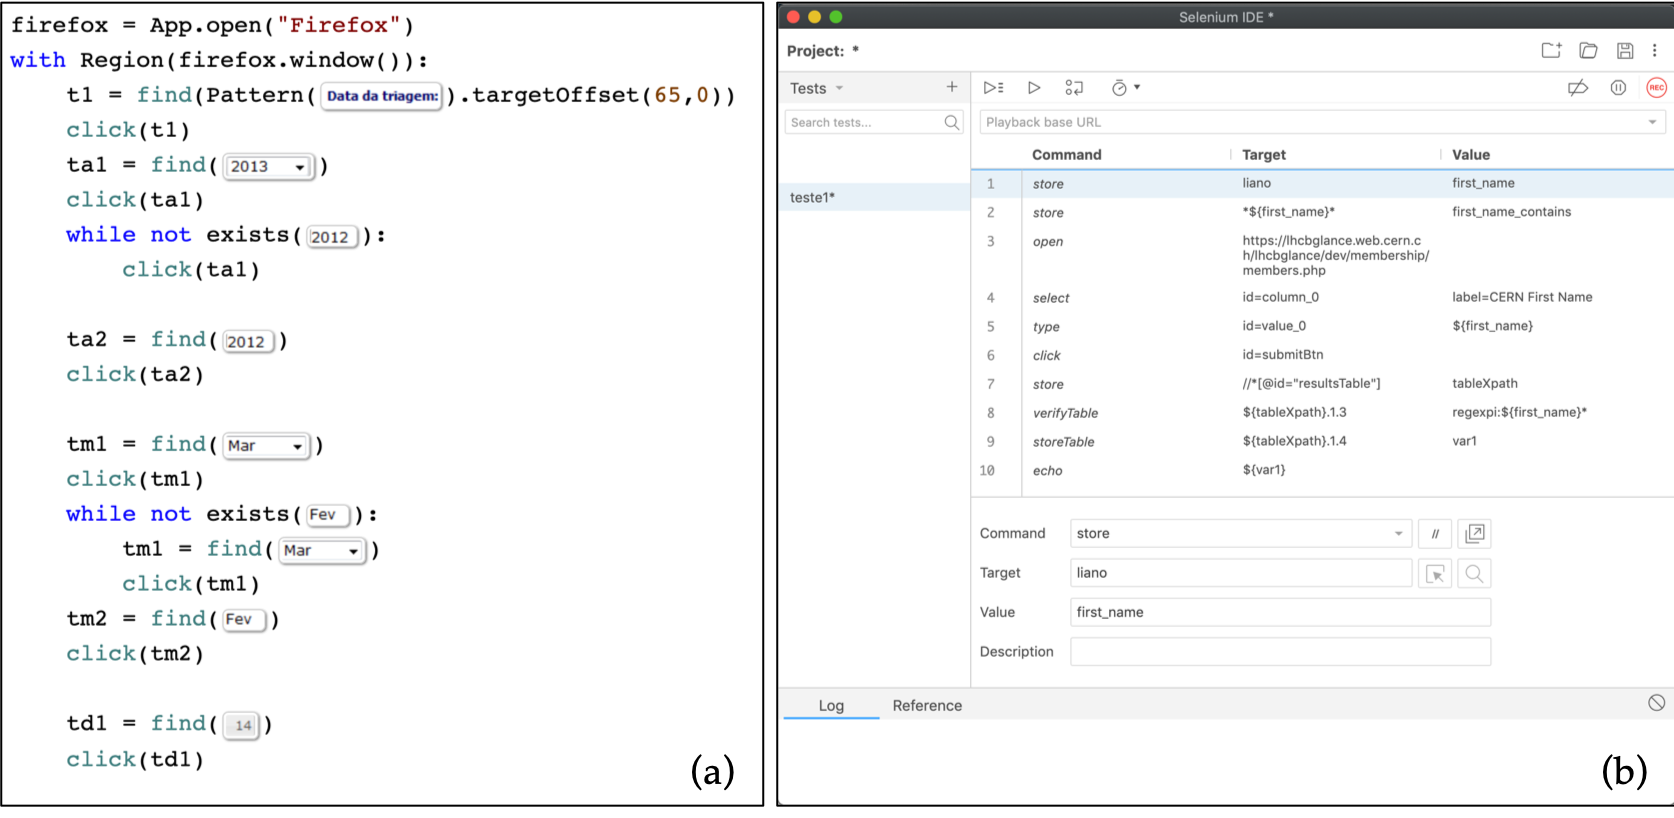
\includegraphics[width=15cm]{source/4-solucao/images/e2e-ferramenta.png}
    \caption{Exemplo de código \emph{Sikuli} em $(a)$, com capturas de tela usadas na lógica do código. Em $(b)$, exemplo de uma instrução de comandos no \emph{Selenium IDE}.}
    \label{fig:e2e-ferramenta}
\end{figure}

Apesar de ambas funcionarem corretamente, nenhuma delas atendia todas as necessidades dos sistemas. O \emph{Sikuli} realiza as asserções de teste por meio de regressão visual com comparação direta de imagens, o que é algo volátil a acusação falsa de erros. Juntando-se isso ao fato de a ferramenta ter perdido grande parte de seus mantenedores, foi desistido do uso da mesma. Já o \emph{Selenium IDE}, apesar de sua praticidade e da sua geração automática de código, não permite lógicas mais complexas, como iterações e condicionais. Concluiu-se que seria preferível escrever os testes diretamente em código, sem captura direta de imagens ou gravação de movimentos, e dessa maneira foi decidido experimentar a ferramenta \emph{Selenium Webdriver}.

O \emph{Selenium Webdriver} é considerado um dos mais famosos \emph{frameworks} de \emph{end-to-end testing} para navegadores. Com ele se torna possível desenvolver testes sofisticados, com lógica de linguagens imperativas, capazes de realizar testes em diferentes sistemas operacionais com navegadores distintos. Disponível em diferentes linguagens, os primeiros protótipos foram feitos na linguagem \emph{Python}. Um exemplo de código de teste realizado se encontra na figura \ref{fig:e2e-ferramenta-2}, em que é verificado se existe um contrato na interface com um nome específico.

\begin{figure}[H]
    \centering
    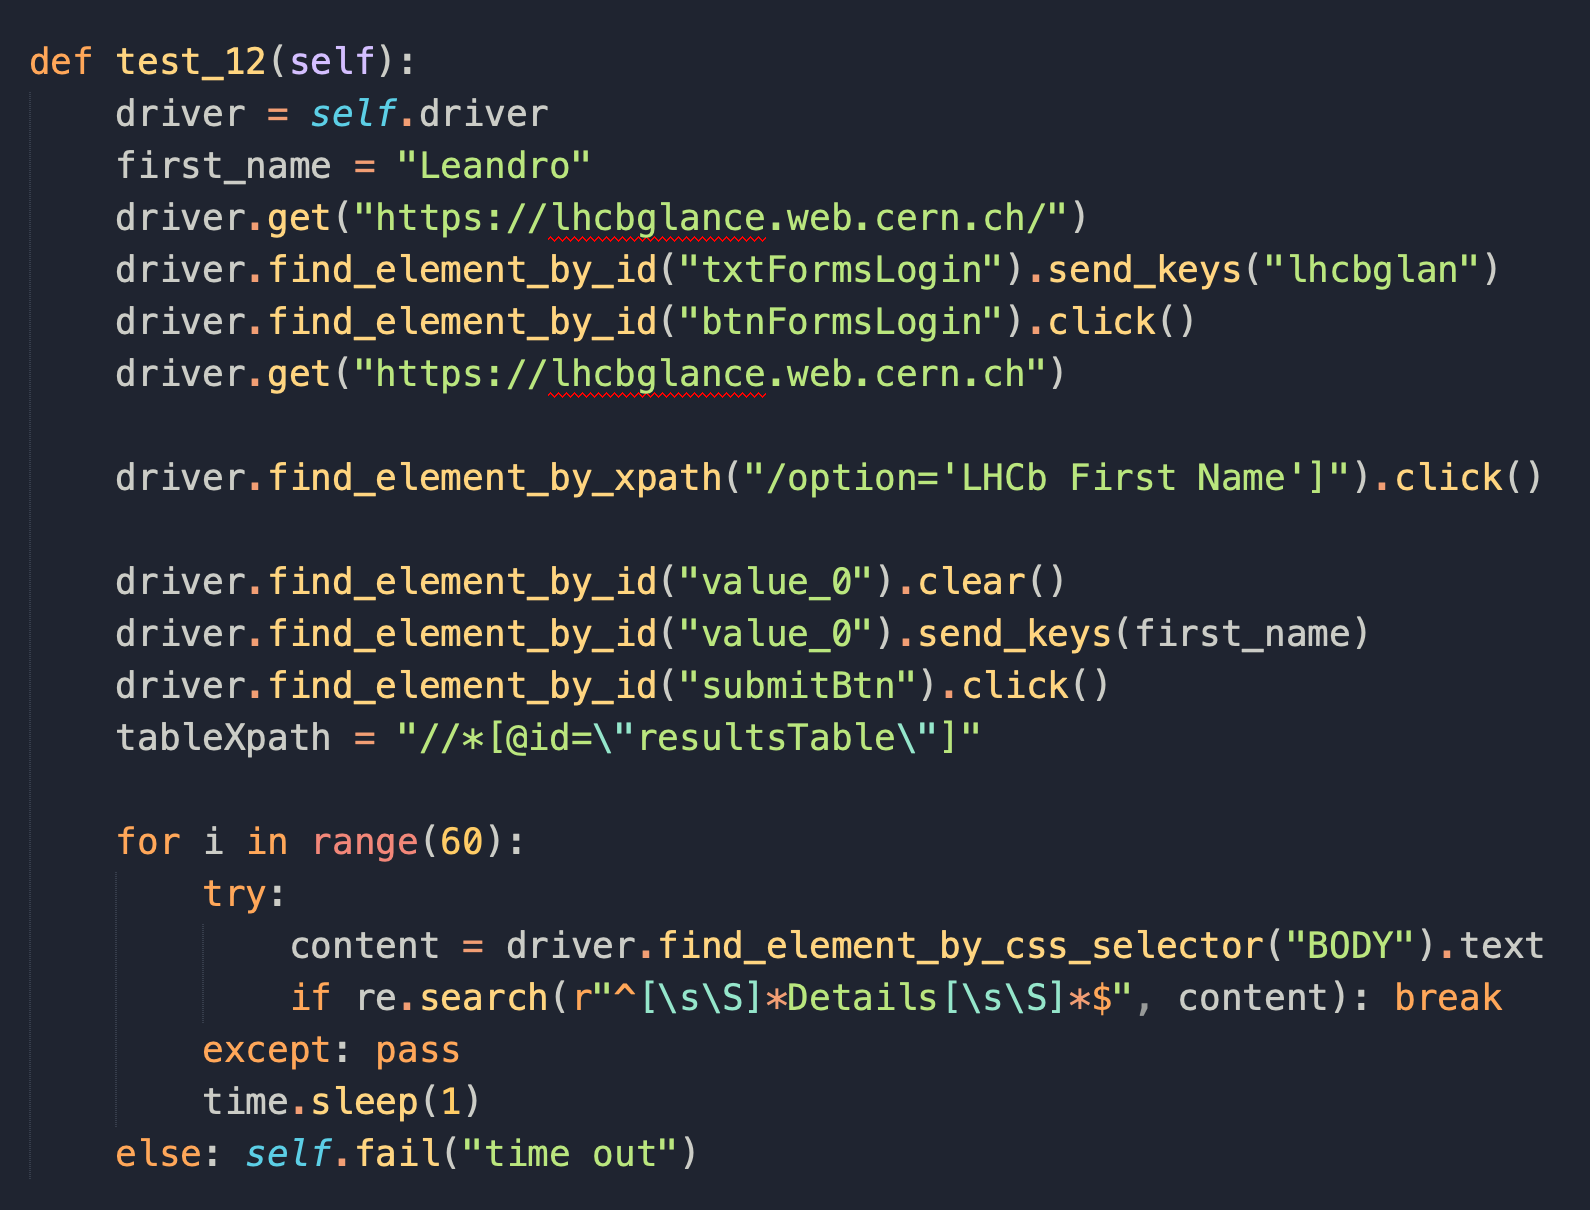
\includegraphics[width=13cm]{source/4-solucao/images/e2e-ferramenta-2.png}
    \caption{Exemplo de código \emph{Python} utilizando o \emph{Selenium Webdriver}.}
    \label{fig:e2e-ferramenta-2}
\end{figure}

\emph{Selenium Webdriver} foi a ferramenta utilizada durante a parte inicial deste trabalho, entretanto não oferece uma solução completa para utilização em ecossistemas mais complexos. Diversos utilitários adicionais não estão presentes no \emph{framework}, como registro de eventos \emph{log}, biblioteca de validações, gerador de relatório, depuração e facilidades a integração contínua. Havia a possibilidade de desenvolver esses complementos, entretanto seria algo que consumiria tempo. Foi então realizada uma nova pesquisa e um novo \emph{framework} foi encontrado, desenvolvido a partir do \emph{Selenium Webdriver}. Chamado de \emph{WebdriverIO}, este foi a escolha final para desenvolvimento deste trabalho.

\hypertarget{implementacao-do-framework-webdriverio}{%
\subsubsection{\texorpdfstring{Implantação do \emph{framework} \emph{WebdriverIO}}{Implementação do framework WebdriverIO}}\label{implementacao-do-framework-webdriverio}}

Este \emph{framework} é uma implementação feita a partir do \emph{Selenium Webdriver}, escrito na linguagem \emph{Javascript} e interpretado pelo mecanismo \emph{Node.js}. Como esta é uma das principais linguagens utilizada pelo grupo de desenvolvedores, a facilidade em escrever código se torna maior do que era com o \emph{Selenium Webdriver} em \emph{Python}. A abstração existente no \emph{WebdriverIO} permite que comandos mais complexos, que implementados em \emph{Selenium} precisam de múltiplas linhas e diversas condicionais para considerar diferentes ambientes, sejam realizados em apenas uma linha. Isso é perceptível principalmente em \emph{watchers}, que são implementações de observadores que aguardam um evento ser realizado antes de dar continuidade com o \emph{script}. \emph{Watchers} são fundamentais para trazer estabilidade aos testes, uma vez que eventos podem ser mais lentos do que esperado, quando por exemplo ocorrem problemas em rede ou no servidor que hospeda a aplicação a ser testada.

Logo no início da configuração do \emph{WebdriverIO}, uma série de ferramentas são oferecidas de acordo com a necessidade. Por meio de um arquivo de configuração, chamado \emph{wdio.conf.js}, é possível definir os parâmetros de execução no teste, como por exemplo na figura \ref{fig:webdriverio}.

\begin{figure}[H]
    \centering
    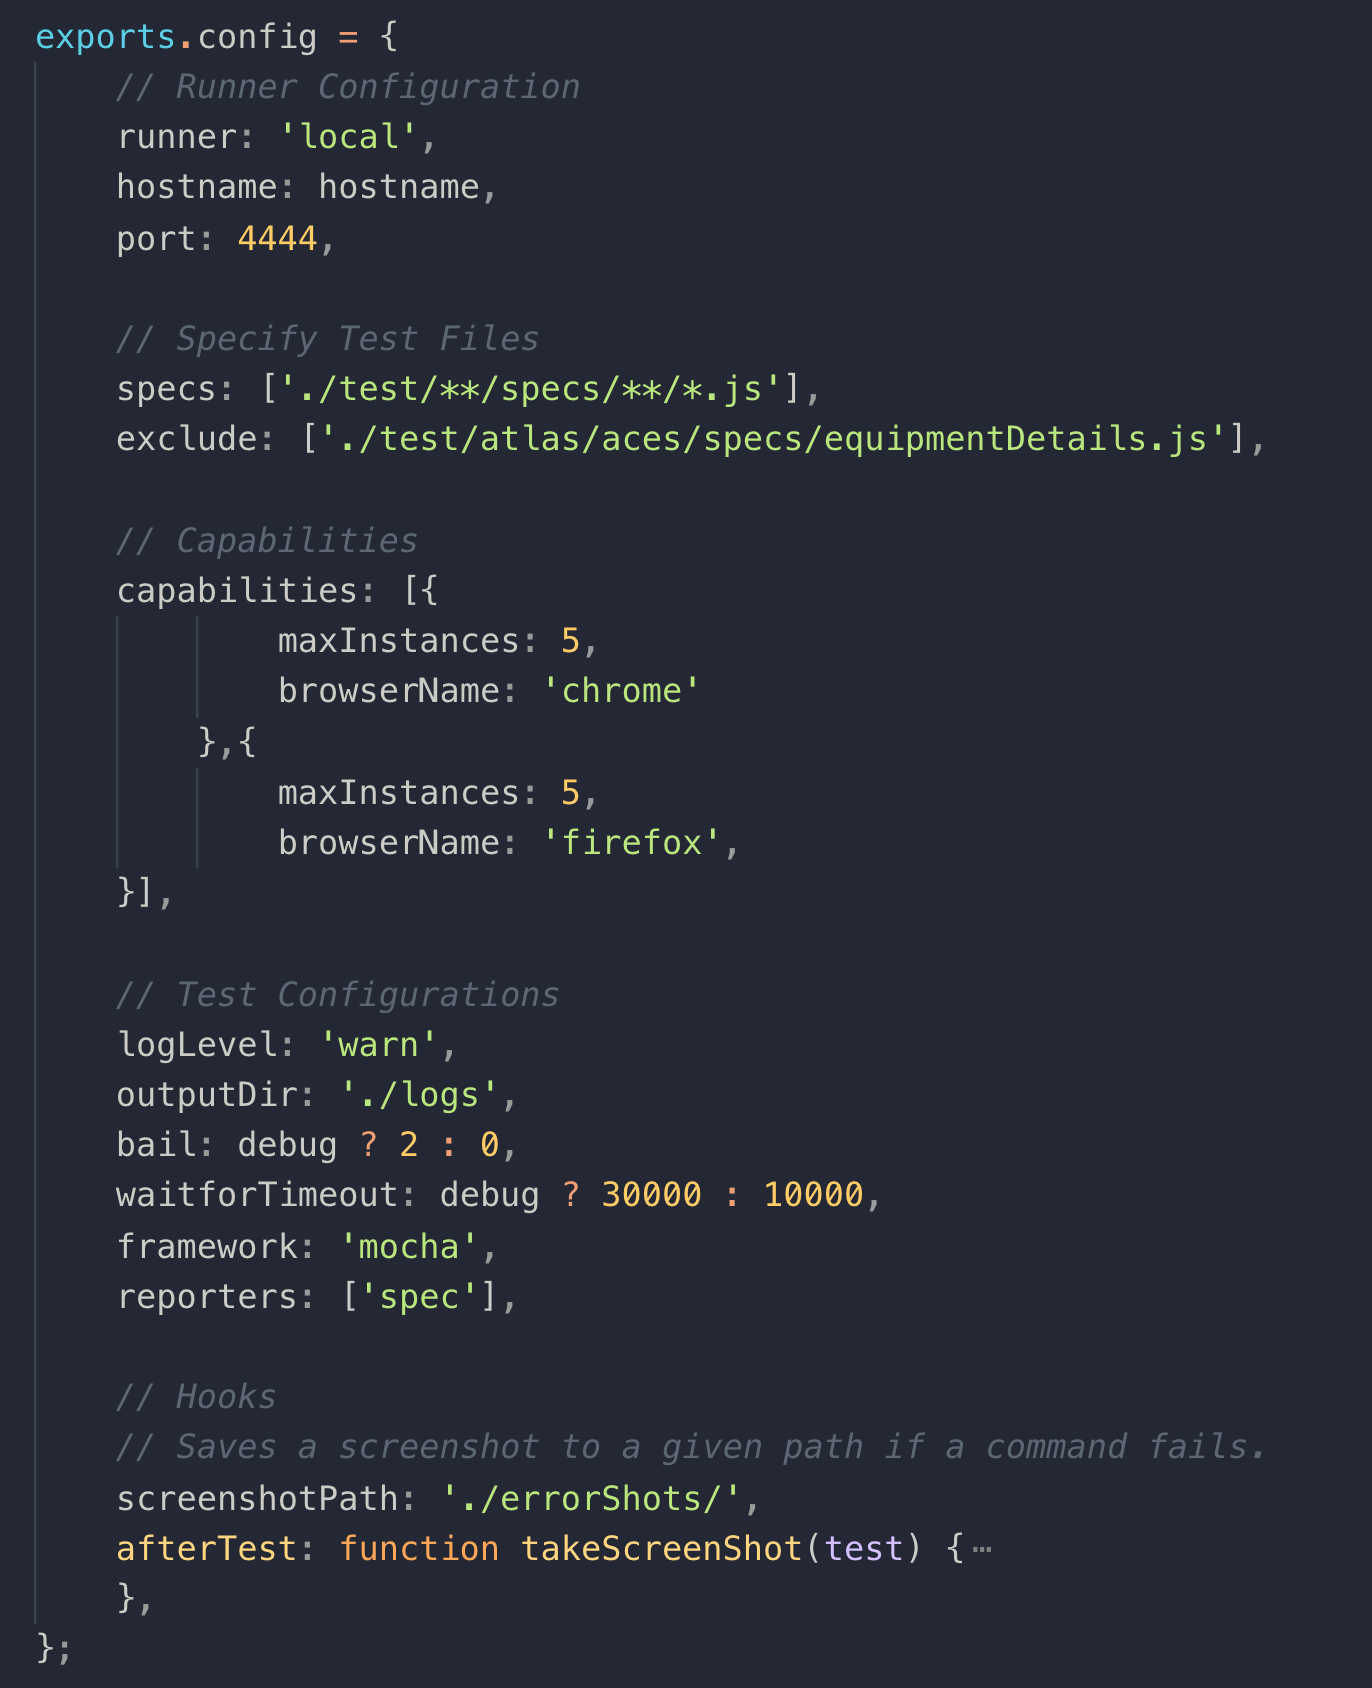
\includegraphics[width=13cm]{source/4-solucao/images/webdriverio.png}
    \caption{Exemplo de arquivo de configuração do \emph{WebdriverIO}.}
    \label{fig:webdriverio}
\end{figure}

Analisando a imagem do arquivo, inicialmente em \emph{Runner Configuration} é possível explicitar em que máquina os testes serão rodados, podendo ser local ou remotamente. \emph{Specify Test Files} permite especificar quais testes executar e quais ignorar. Por \emph{Capabilities} é viabilizado balancear em quantas instâncias de quais navegadores os testes executarão em paralelo. \emph{Test Configurations} define configurações gerais, como verbosidade de \emph{log}, tempo máximo de duração do teste com os \emph{timeouts}, tolerância com testes falhos em \emph{bail}, e escolha de ferramentas adicionais, como \emph{framework} auxiliares de testes e \emph{reporters} que geram os relatórios finais. Por fim, há os \emph{hooks}, que permitem realizar tarefas adicionais durante o ciclo de execução, como por exemplo tirar uma \emph{screenshot} da página ao fim de um teste quando ocorre um erro.

\emph{WebdriverIO} possui embutido recursos avançados de escrita de código. Por exemplo o \emph{tradutor Babel} para conversão de código, permitindo o uso das funcionalidades mais recentes do \emph{Javascript}, e o validador \emph{typescript}, que permite tipificar a linguagem. O \emph{framework} também é compatível com serviços de execução de testes em nuvem, como o \emph{Sauce Labs}, e depuração avançada, com a interface \emph{REPL} que permite inspecionar o teste no momento de execução.

Com essa alta capacidade de customização e integrações disponíveis, foi preparado um ambiente inicial para uso da ferramenta, e testes passaram a ser escritos. O crescimento do número de testes e de funcionalidades compartilhadas, deu início a um novo \emph{framework}, que será mencionado adiante, construído a partir do \emph{WebdriverIO} e voltado para interfaces em \emph{Fence}.

\hypertarget{implementacao-e-design-do-fate}{%
\subsubsection{\texorpdfstring{Implementação e \emph{design} do \emph{Fate}}{Implementação e design do Fate}}\label{implementacao-e-design-do-fate}}

O \emph{framework} \emph{Fate}, segue princípios próximos dos utilizados no \emph{FUnit}. Um híbrido de paradigmas funcional e orientado a objetos é utilizado, com também aplicação dos princípios \emph{SOLID} e abstração em arquivos de configuração.

\begin{figure}[H]
    \centering
    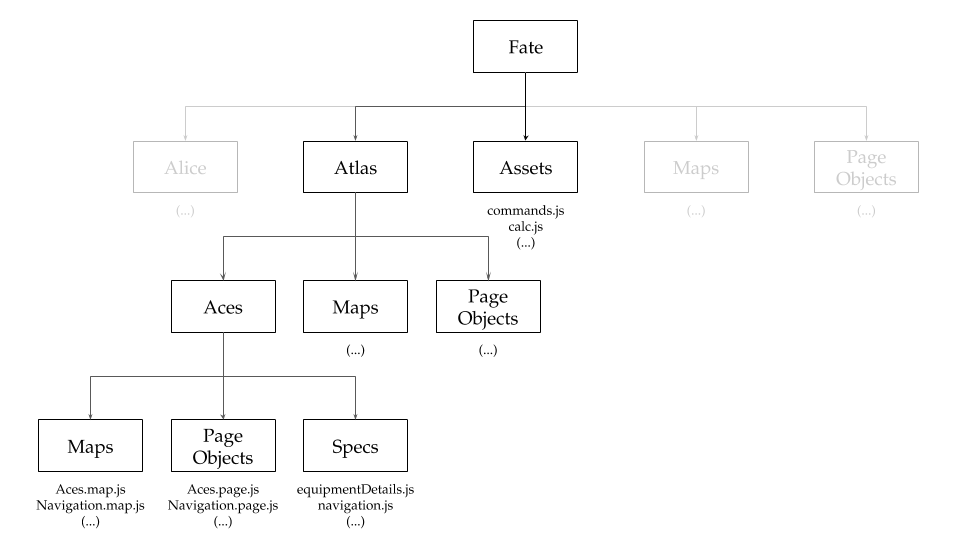
\includegraphics[width=15cm]{source/4-solucao/images/fate-esq-2.png}
    \caption{Estrutura de arquivos do \emph{Fate}, categorizados basicamente em \emph{Specs}, \emph{Page Objects} e \emph{Maps}. À medida que se ramifica, os arquivos abaixo possuem acesso às propriedades dos acima.}
    \label{fig:fate-esq-2}
\end{figure}

Como ilustrado na figura \ref{fig:fate-esq-2}, a estrutura que o \emph{Fate} possui é hierarquizada em diretórios. No topo, há a divisão em experimentos, \emph{Atlas} e \emph{Alice}, e a existência do diretório \emph{Assets}, onde se encontram bibliotecas globais com funções que auxiliam a escrita de testes, como comandos adicionais para simular ações comuns de usuários nos sistemas \emph{Fence} e operações matemáticas regulares nos testes.

Dentro do diretório \emph{Atlas}, é possível ver uma segunda divisão baseada em sistemas, como o \emph{ACES}. No interior do diretório do sistema, é possível ver os diretórios \emph{Maps}, \emph{Page Objects} e \emph{Specs}. Em \emph{Specs}, se encontram os testes que serão executados, executando as interações desejadas com a interface a ser testada. Estas interações são disponibilizadas pelos \emph{Page Objects}, que se responsabilizam em conter a lógica e as interações disponíveis para cada interface disponibilizada para teste. Os arquivos \emph{Maps} armazenam informações adicionais de configuração do objeto, como localizadores, que serão utilizados pelos \emph{Page Objects}.

Essa organização se baseia em um padrão de \emph{design} chamado de \emph{page object pattern}. Esse \emph{design} defende a ideia de cadeia de responsabilidades, na qual se separa o que precisa ser testado de como precisa ser testado. Isso torna mais simples o reaproveitamento de código entre testes, principalmente quando possuem páginas web em comum. Portanto o \emph{page object pattern} recomenda a implementação de um objeto que represente a sua página, possuindo propriedades e métodos próprios que definem as possibilidades de interação pelos testes. Dessa forma, não é de responsabilidade do teste em implementar a lógica de interação, cabendo apenas importar o objeto \emph{page} o qual deseja testar e utilizar as interações disponíveis. Na próxima seção será ilustrado um caso de uso desta estratégia.

É frequentemente utilizado no \emph{Fate} o princípio da herança. \emph{Page Objects} e \emph{Maps} são definidos ao longo de toda a hierarquia do \emph{framework}, de forma que à medida que se desce um nível de diretório, \emph{Page Objects} e \emph{Maps} deste nível herdam as funcionalidades dos respectivos diretórios pais. Este é um princípio inspirado no \emph{framework Fence}, que também realiza a mesma prática. Portanto, como visto no exemplo da figura \ref{fig:fate-esq-2}, \emph{Page Objects} e \emph{Maps} possuem acesso as funcionalidades adicionais dos diretórios de mesmo nome presentes em \emph{Atlas} e na raiz do \emph{Fate}.

\hypertarget{tecnologias-e-caso-de-uso}{%
\subsubsection{Tecnologias e caso de uso}\label{tecnologias-e-caso-de-uso}}

Em relação às tecnologias utilizadas, o \emph{Fate} possui um conjunto abrangente. Além do \emph{WebdiverIO}, sua arquitetura faz uso também de \emph{frameworks} e bibliotecas adicionais, como presente no fluxograma da figura \ref{fig:fate-framework}. Diferentemente do \emph{FUnit} que depende unicamente do \emph{phpunit}, na linguagem \emph{Javascript} há um número maior de opções que permitem uma maior customização da aplicação.

\begin{figure}[H]
    \centering
    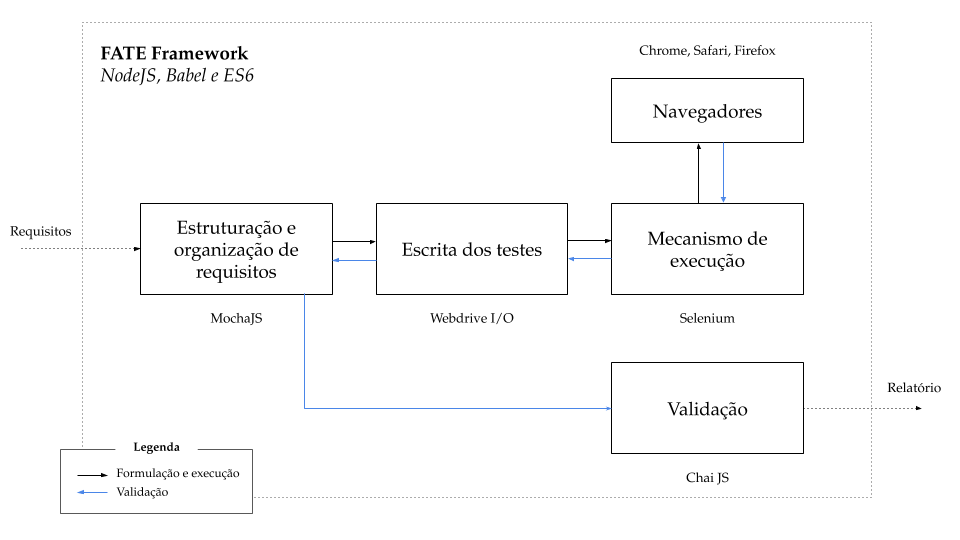
\includegraphics[width=14.5cm]{source/4-solucao/images/fate-framework.png}
    \caption{Funcionamento detalhado do \emph{Fate}. Os testes são escritos, executados e validados após a estruturação dos requisitos.}
    \label{fig:fate-framework}
\end{figure}

Inicialmente os requisitos são expressados no formato exigido pelo \emph{framework Mochajs}, que tem como responsabilidade estruturar e administrar a execução de testes. Ele associa os requisitos em \emph{test cases}, aciona a rotina em \emph{WebdriverIO} respectiva a cada \emph{test case}, compara o resultado obtido com a biblioteca de validação, e finalmente invoca o gerador de relatórios escolhido. Na figura \ref{fig:aces-example}, há a página web \emph{navigation} do sistema \emph{ACES}, que possui a esquerda uma lista de itens utilizados no exemplo de teste a seguir.

\begin{figure}[H]
    \centering
    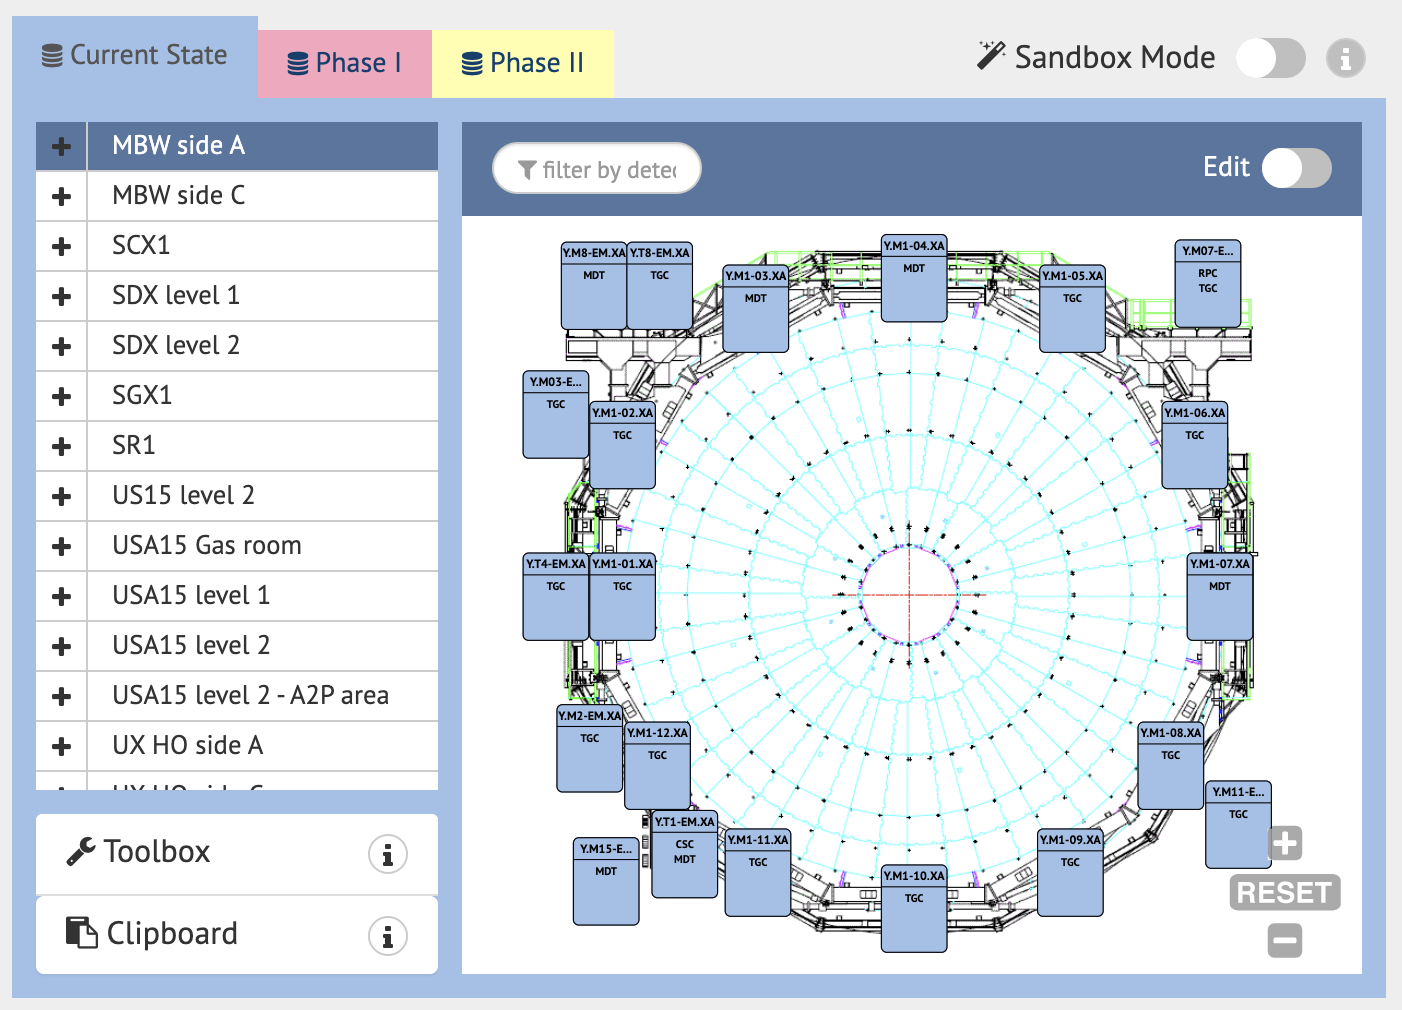
\includegraphics[width=11.75cm]{source/4-solucao/images/aces-example.png}
    \caption{Captura de tela do sistema \emph{ACES}, com a lista de itens à esquerda, que são o objeto de exemplo do teste.}
    \label{fig:aces-example}
\end{figure}

O requisito extraído do plano de testes é descrito no \emph{test case} da \emph{Spec} \emph{navigation}, como no exemplo da figura \ref{fig:fate-spec}, em que quando se clica na página em um item aleatório da lista, o título da página deve ser atualizado com o nome do item. Em seguida, se dá início a escrita do teste, onde é utilizado o \emph{Page Object} \emph{Navigation} para requisitar as interações necessárias para o prosseguimento do teste.

\begin{figure}[H]
    \centering
    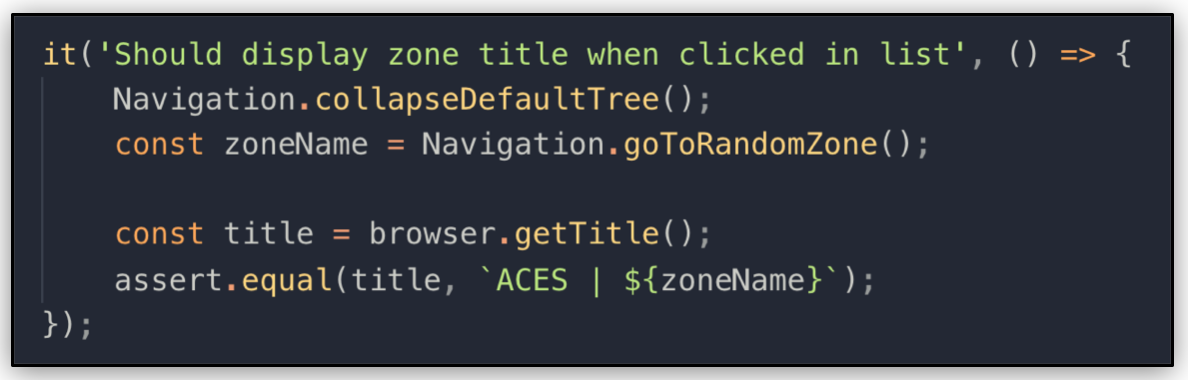
\includegraphics[width=13cm]{source/4-solucao/images/fate-spec.png}
    \caption{\emph{Spec} realizando os pedidos ao \emph{Page Object} e validando.}
    \label{fig:fate-spec}
\end{figure}

No conteúdo do \emph{Page Object}, na figura \ref{fig:fate-page-object}, é possível ver a definição da série de passos necessários para atender o pedido do \emph{Spec}. No método \emph{collapsedDefaultTree} é pedido ao \emph{WebdriverIO} que aguarde a existência do elemento \emph{htCollapsedNode}, que contém a lista de itens, até o limite de tempo \emph{timeout}, acusando erro se ultrapassado. Após isso, é enviado o comando \emph{click}, que representa o clique de um \emph{mouse}, para colapsar a lista. O \emph{WebdriverIO} recebe estes comandos, traduz e envia para o \emph{Selenium} por meio da \emph{API}, que realiza as respectivas ações no navegador, como por exemplo \emph{Chrome}, \emph{Firefox} ou \emph{Safari}.

\begin{figure}[H]
    \centering
    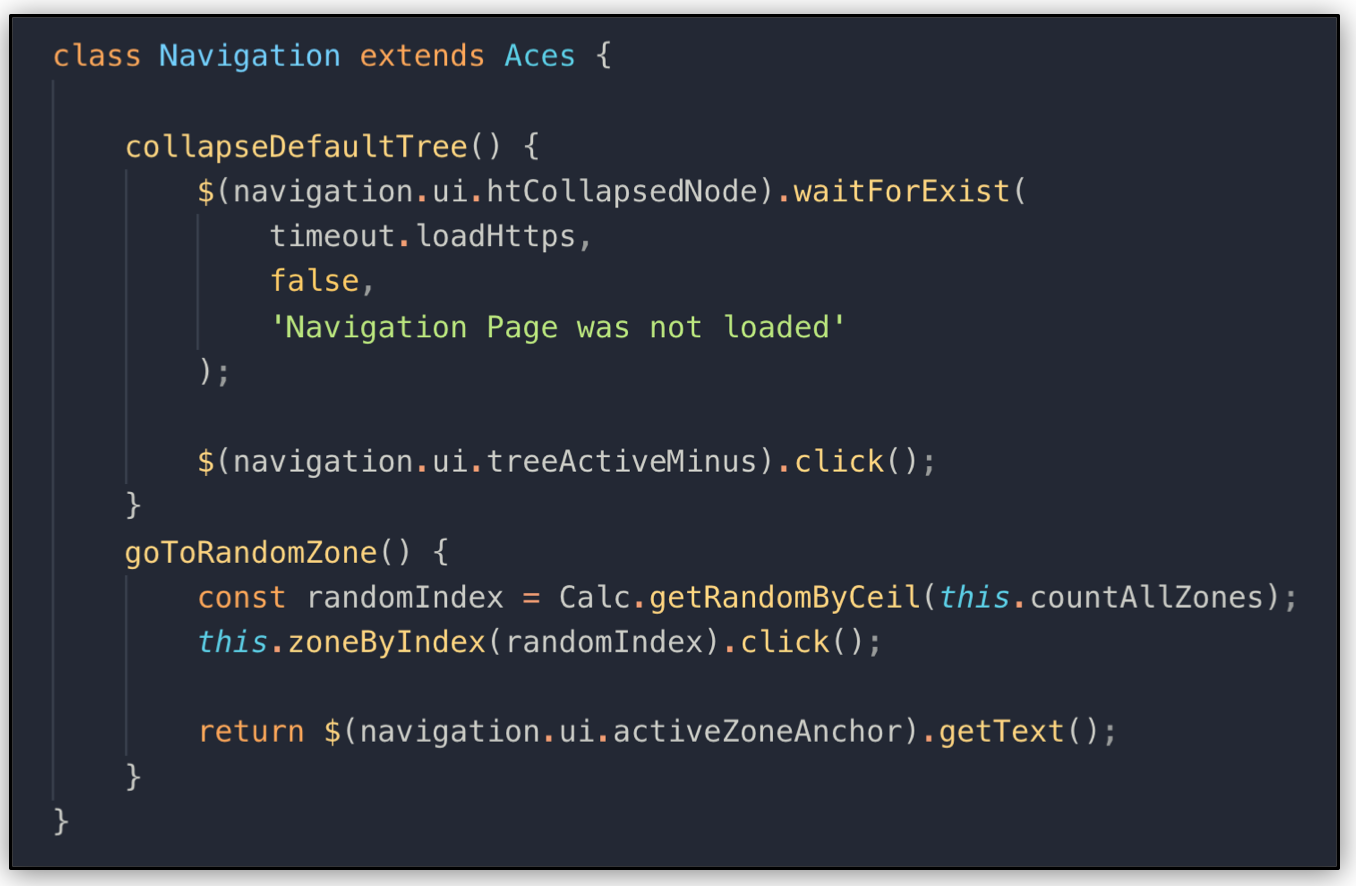
\includegraphics[width=14.5cm]{source/4-solucao/images/fate-page-object.png}
    \caption{\emph{Page Object} contendo a lógica de ações disponíveis na interface.}
    \label{fig:fate-page-object}
\end{figure}

Realizadas as ações, a execução é retomada no \emph{Page Object}, que retorna o fim da interação para o \emph{Spec} original. É válido notar também que ao longo do código do \emph{Page Object} \emph{Navigation}, diversas propriedades do objeto \emph{navigation.ui} são utilizadas, as quais pertencem ao arquivo \emph{Maps}. Este arquivo, ilustrado na figura \ref{fig:fate-maps}, funciona como um dicionário, fornecendo informações de localização de elementos na página e seus atributos.

\begin{figure}[H]
    \centering
    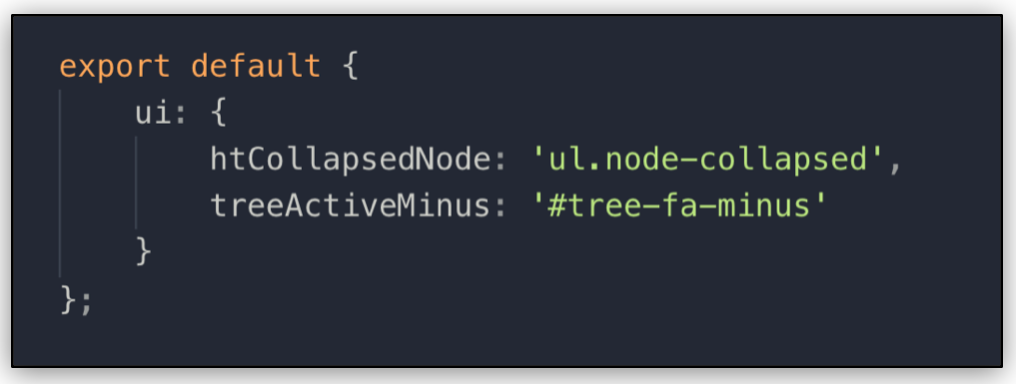
\includegraphics[width=11cm]{source/4-solucao/images/fate-maps.png}
    \caption{\emph{Maps} com a localização dos elementos usados pelo \emph{Page Object}.}
    \label{fig:fate-maps}
\end{figure}

Finalizadas as interações desejadas com a página, tem-se a validação na última linha da \emph{Spec}. No exemplo mostrado, é utilizado o método \emph{assert.equal}, disponibilizado pela biblioteca \emph{Chaijs}. Esta biblioteca permite diversos tipos de validações para diferentes estruturas de dados, facilitando as verificações do teste. No caso da \emph{FUnit}, as validações disponíveis no \emph{phpunit} são mais limitadas, tendo sido necessária a implementação de mais opções de validação.

Este processo descrito é repetido para cada \emph{test case} do arquivo \emph{Spec}, e a partir do momento em que todos os arquivos são executados ou interrompidos em caso de erro, um relatório é então gerado. Atualmente são utilizados três tipos diferentes de relatórios, um para cada situação, exemplificadas na figura \ref{fig:allure-report}. O relatório \emph{Dot Reporter} é compacto e usado principalmente para verificações rápidas de regressão enquanto se desenvolvem novos testes. No caso do relatório \emph{Spec Reporter}, ele é utilizado principalmente durante as \emph{pipelines} da integração contínua, e fornece informações mais detalhadas sobre a execução dos testes também em linha de comando. E finalmente há o relatório \emph{Allure Reporter}, que se trata de uma página web e possui uma análise gráfica criteriosa dos testes, sendo utilizado principalmente para situações mais formais, como apresentações e auditorias.

\begin{figure}[H]
    \centering
    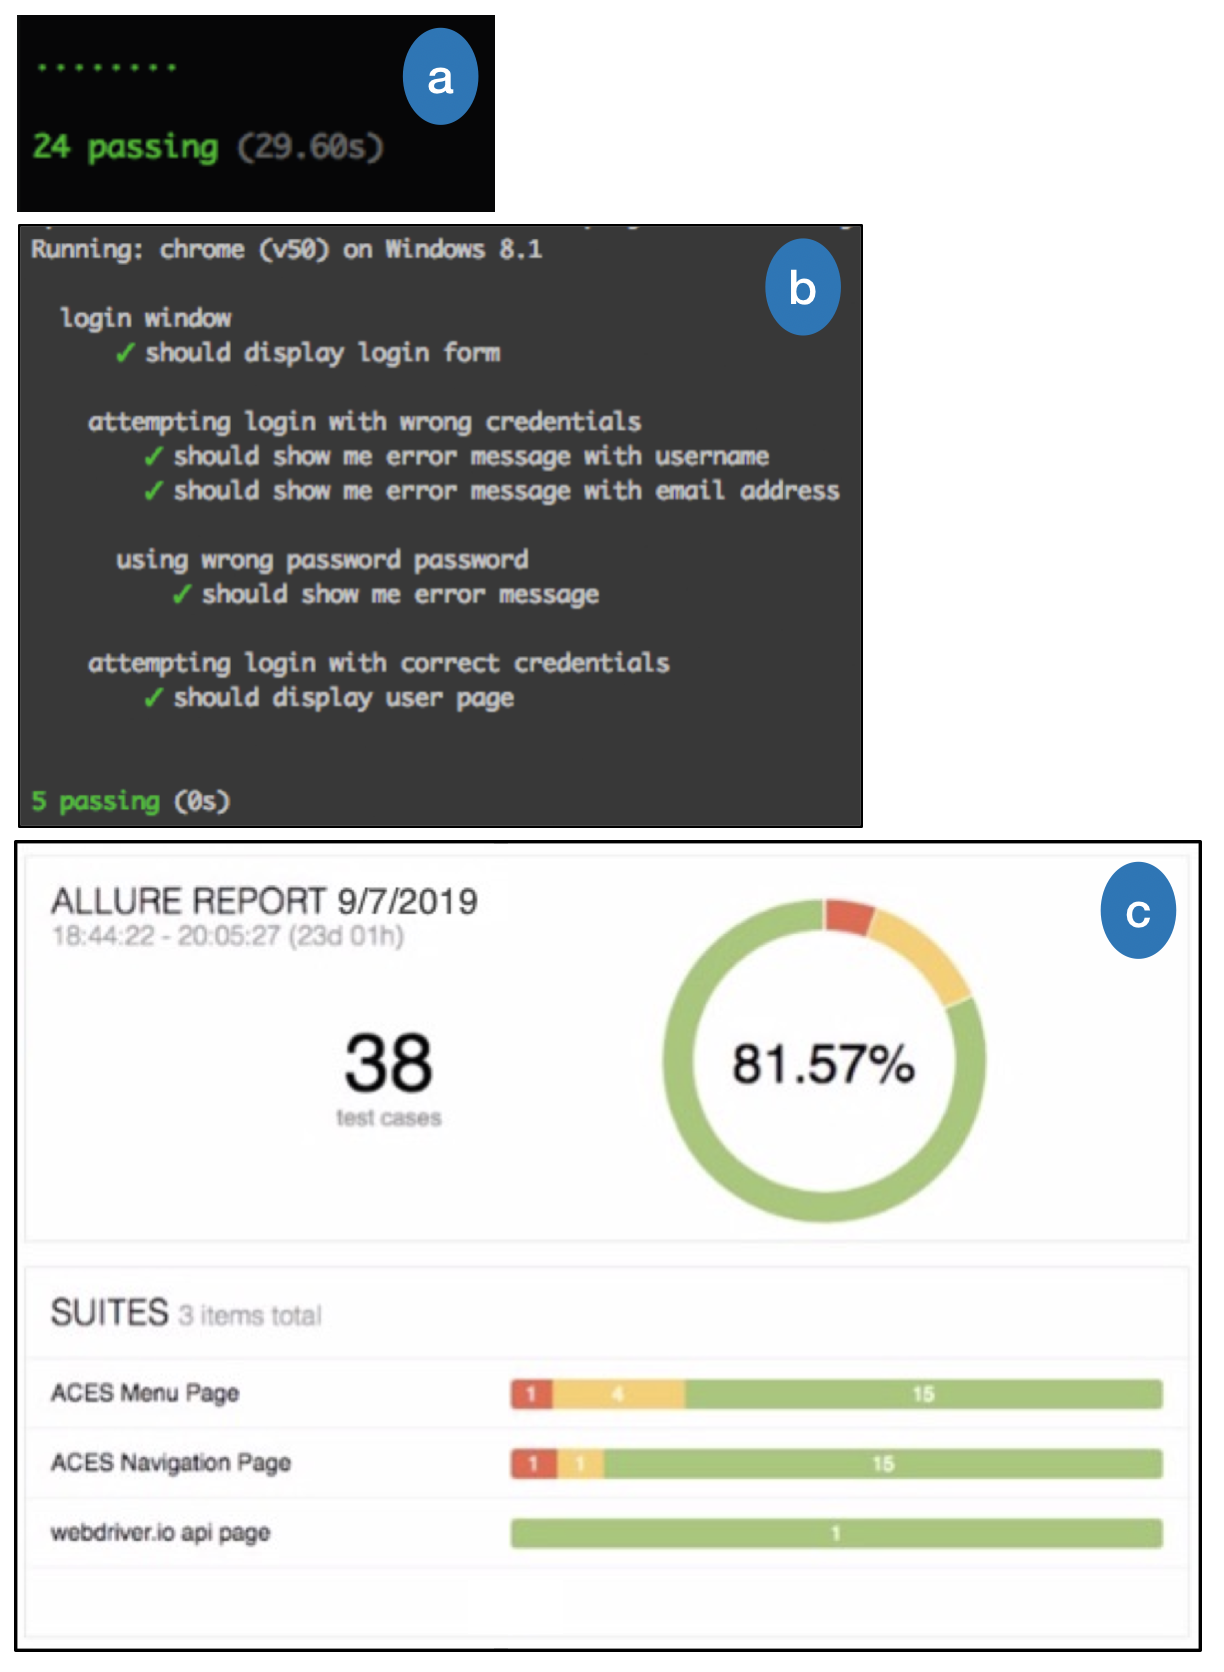
\includegraphics[width=13cm]{source/4-solucao/images/fate-reporters-vertical.png}
    \caption{Exemplos de relatórios gerados pelo \emph{Fate}. \emph{Dot} em $(a)$, \emph{Spec} em $(b)$ e \emph{Allure} em $(c)$.}
    \label{fig:allure-report}
\end{figure}

\hypertarget{teste-de-regressao-visual}{%
\subsubsection{Teste de regressão visual}\label{teste-de-regressao-visual}}

Com a disponibilização recente da nova ferramenta \emph{ResembleJS} pelo \emph{WebdriverIO}, se tornou possível também a realização de testes de regressão visual. Estes testes realizam comparação direta de imagens, o que é útil em certos casos, apesar de serem testes que exigem mais processamento. O comportamento é semelhante ao da ferramenta \emph{Sikuli} mencionada anteriormente. Entretanto, diferentemente do \emph{Sikuli}, a integração com o \emph{ResembleJS} já é nativa e compatível com o ambiente de desenvolvimento do \emph{Fate}, exigindo menos esforço para ser utilizada.

A figura \ref{fig:aces-example-2} disponibiliza um exemplo de seu funcionamento. Na imagem extraída da página de \emph{navigation} do \emph{Aces}, é possível observar um desenho com pequenos retângulos posicionados ao seu redor. Estes retângulos são chamados de \emph{racks} e representam painéis de eletrônicos posicionados fisicamente em uma seção transversal do detector \emph{Atlas}, no subsolo do \emph{CERN}. Estes \emph{racks} não podem ser movimentados ou removidos, portanto, um teste de regressão visual foi desenvolvido para eles. Ao remover o \emph{rack} \emph{Y.M1-05.XA} e executar o teste, é possível ver que o teste destaca a diferença entre a imagem de referência e a obtida, acusando o erro. Assim é possível garantir a confiabilidade do mapa em questão.

\begin{figure}[H]
    \centering
    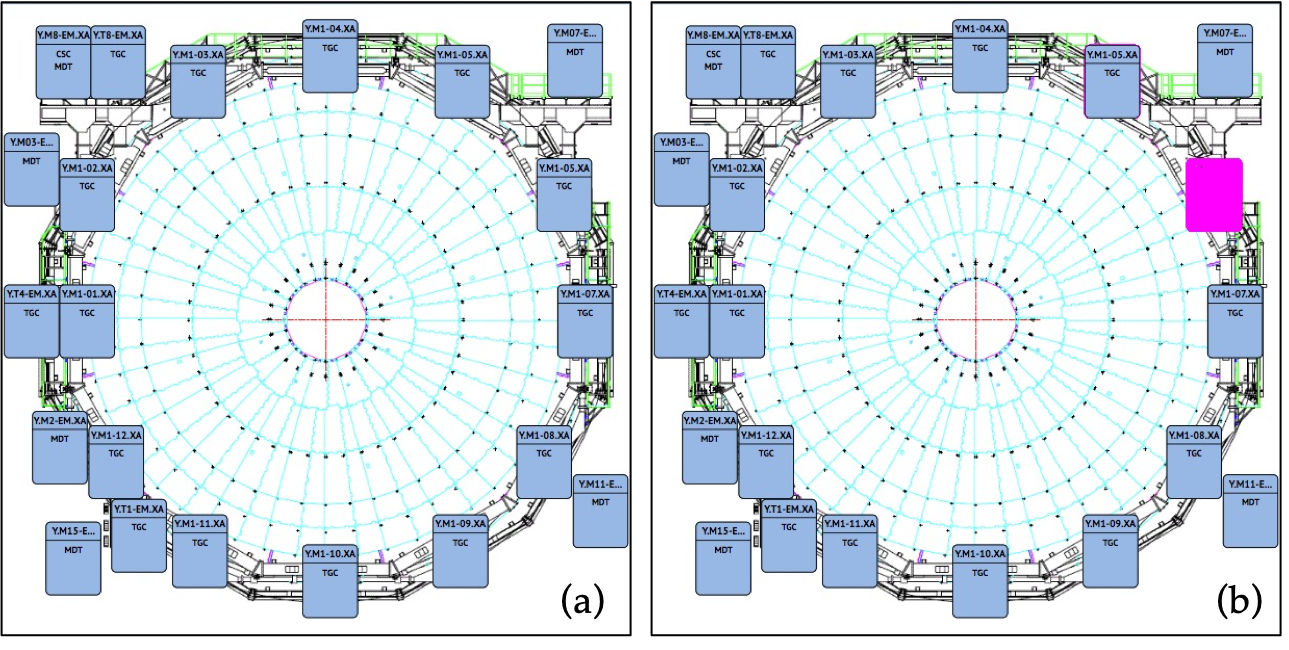
\includegraphics[width=13cm]{source/4-solucao/images/aces-example-2.png}
    \caption{Exemplo de teste de regressão visual. O teste identificou a ausência de um \emph{rack} na área em rosa.}
    \label{fig:aces-example-2}
\end{figure}

O desenvolvimento dos testes unitários utilizando \emph{FUnit} e dos testes \emph{e2e} com o \emph{Fate} mostrou a importância da elaboração de um ambiente de execução automática conforme a demanda. Isso motivou o desenvolvimento da integração contínua para os \emph{frameworks}, que será discutida na próxima seção.
